\documentclass[letterpaper]{article} % DO NOT CHANGE THIS
\usepackage[submission]{aaai2027}  % DO NOT CHANGE THIS
\usepackage[hyphens]{url}  % DO NOT CHANGE THIS
\usepackage{graphicx} % DO NOT CHANGE THIS
\urlstyle{rm} % DO NOT CHANGE THIS
\def\UrlFont{\rm}  % DO NOT CHANGE THIS
\usepackage{natbib}  % DO NOT CHANGE THIS AND DO NOT ADD ANY OPTIONS TO IT
\usepackage{caption} % DO NOT CHANGE THIS AND DO NOT ADD ANY OPTIONS TO IT
\frenchspacing  % DO NOT CHANGE THIS
\usepackage{booktabs}
\usepackage{array}
\usepackage{amsmath,amssymb,amsthm}
\usepackage{pgfplots}
\pgfplotsset{compat=1.18}
\usepgfplotslibrary{groupplots}
\usetikzlibrary{arrows.meta,positioning,calc}

\pdfinfo{
/TemplateVersion (2027.1)
}

\setcounter{secnumdepth}{2}

\definecolor{cD}{HTML}{0072B2}
\definecolor{cE}{HTML}{D55E00}
\definecolor{cS}{HTML}{009E73}
\definecolor{cP}{HTML}{56B4E9}
\definecolor{cF}{HTML}{CC79A7}

\newtheorem{theorem}{Theorem}
\newtheorem{proposition}{Proposition}
\newtheorem{corollary}{Corollary}
\newtheorem{lemma}{Lemma}
\theoremstyle{definition}
\newtheorem{definition}{Definition}
\newtheorem{remark}{Remark}

\newcommand{\hull}{\operatorname{hull}}
\newcommand{\core}{\operatorname{core}}
\newcommand{\dD}{\mathsf{D}}
\newcommand{\dE}{\mathsf{E}}
\newcommand{\dS}{\mathsf{S}}
\newcommand{\cC}{\mathcal{C}}
\newcommand{\cQ}{\mathcal{Q}}
\newcommand{\cS}{\mathcal{S}}
\newcommand{\cD}{\mathcal{D}}
\newcommand{\Valarm}{V_{\mathrm{alarm}}}
\newcommand{\Vmin}{V_{\min}}
\newcommand{\mfl}{m_{\mathrm{fl}}}

\title{No Viable Winner: Competitive Selection, Captured Correction,\\ and the Necessity of Cooperation in AI Development}
\author{Anonymous Submission}
\affiliations{}

\begin{document}

\maketitle

\begin{abstract}
Frontier AI is developed in a race whose participants depend on shared conditions, such as functioning institutions, a reliable information environment and the capacity to detect and correct error, and whose winners help build the evaluations and rules that judge the next round. We ask what this arrangement selects for, and show under explicit, testable conditions that it cannot correct itself. Selection on relative performance does not register conditions that all participants share, so restraint that sustains them is displaced whatever the participants value; the more weight the contest places on winning, the sooner this holds. The obvious remedy, a corrector that makes costs return to those who cause them, is itself part of the selection environment: control over it is selected in the largest participants, and investment in correcting it is selected against. As AI lowers the cost of control, the independent correction needed to keep evaluation uncaptured rises, and correction that grows at less than half that rate is overtaken; after that, harm can cross a critical floor before any alarm. Each remedy now relied on leaves a necessary condition unmet. The conditions of any viable trajectory can be established only jointly, and they leave every participant better off. In this model, cooperation is not an ideal but a necessity.
\end{abstract}

\section{Introduction}

``But who will guard the guardians?'' \citep{hurwicz2008}. Every serious proposal for making advanced AI safe adds a guardian: independent evaluators, standards and certification, safety institutes, AI systems that judge other AI systems, liability and regulation. Each assumes that the guardian stays independent of what it guards. Meanwhile frontier development is organized and financed as a contest, and leading governments describe it as ``a race to achieve global dominance'' \citep{whitehouse2025} or as international competition in which first-mover advantage is to be seized \citep{statecouncil2017}. This paper asks what such a race does to the conditions its participants share, and to the guardians meant to protect them.

Our answer has three parts. \emph{First order:} competition selects on relative performance, and a condition that every participant shares cancels from every comparison; restraint that sustains it is therefore displaced whatever the participants value, and the more a contest rewards winning, the sooner (Section~\ref{sec:first}). \emph{Second order:} the remedy is a corrector that makes costs return to whoever causes them, but the corrector is itself a selection environment into which success converts; control over it is selected in the largest participants, and investment in correcting it is selected against (Section~\ref{sec:second}). \emph{Rate and evidence:} AI lowers the cost of control, so the independent correction required to keep evaluation uncaptured rises; once it is outpaced, captured evaluation can let harm cross a critical floor before any alarm fires (Sections~\ref{sec:second}--\ref{sec:silent}). Together these show why the trajectory of winning fails (Theorem~\ref{thm:fail}), why each remedy now relied on fails with it (Table~\ref{tab:remedies}), and what any viable trajectory requires (Theorem~\ref{thm:invariants}). The requirements bind every participant at once and raise every participant's absolute payoff, so cooperation follows as a necessity rather than a hope (Corollary~\ref{cor:coop}).

\paragraph{Method.} Every claim is a conditional statement proved with standard tools: replicator and payoff-monotone dynamics, the Price equation, linear public-goods games and comparison theorems for monotone systems. Nothing depends on attributing motives. A reader who rejects a conclusion must therefore reject a condition. We state each condition as something observable and pair it with present evidence and with the observations that would refute it (Section~\ref{sec:evidence}). The analysis is not a forecast of catastrophe. It sorts trajectories into viable and non-viable ones.

\paragraph{Contributions.} (1) A first-order result connecting relative selection, the weight a contest places on winning, and the viability of a shared host. (2) Second-order results in one model: selection for control over correctors, with a size threshold; correction as a selected-against public good; and the minimum rate of independent correction, which must grow at least half as fast as AI lowers the cost of control. (3) Conditions under which captured evaluation lets harm cross a floor unseen. (4) A theorem that the trajectory of winning fails, with the failure mode of seven current remedies, and a theorem stating invariants that are indispensable and jointly sufficient in the model, from which the necessity of cooperation follows.

\paragraph{Statement of Contributions.} The results are new in this setting and are obtained with standard tools, which we cite; the first-order mechanism is classical, and our contribution lies in connecting it to the selection of correctors, to the rate at which AI changes the cost of control, and to the conditions for viable trajectories. Some conceptual antecedents appeared in informal, non-peer-reviewed essays. All formal content is new and unpublished.

\section{Related Work}\label{sec:related}

\paragraph{Races and cooperation in AI.} Competitive pressure can erode safety investment \citep{armstrong2016,askell2019,dafoe2020}; AI can cause harm by changing incentives \citep{zwetsloot2019}, gradually displacing human influence \citep{christiano2019,kulveit2025}, or through multi-principal dynamics that per-system alignment leaves untouched \citep{critch2020,critch2021,hendrycks2023,hammond2025}. We add the selection of correctors and a rate condition.

\paragraph{Relative selection.} Selection rewards relative, not absolute, performance \citep{alchian1950}; in finite populations evolutionary stability maximizes relative payoff \citep{schaffer1988}, and imitation leads to relative-payoff-maximizing behavior \citep{vegaredondo1997}. Positional concern undermines shared goods \citep{hirsch1976,frank1985}. The commons and its governance \citep{hardin1968,olson1965,ostrom1990}, the second-order free-rider problem of sanctioning \citep{oliver1980,yamagishi1986,heckathorn1989}, which reputation can stabilize under some conditions \citep{panchanathan2004}, and environmental feedback in evolutionary games \citep{weitz2016,tilman2020} supply our first-order and correction results; viability theory supplies the language of floors \citep{aubin1991,rockstrom2009}.

\paragraph{Guardians, capture and certification.} Regulators can be captured \citep{stigler1971,laffont1991,dalbo2006,carpenter2013}, including without intent \citep{kwak2014}; a monopoly certifier may reveal little \citep{lizzeri1999}, and raters paid by those they rate face conflicts that inflate ratings \citep{bolton2012}; rankings reshape what they measure \citep{espeland2007,campbell1979,manheim2018}. Niche construction is selected when its benefits are appropriable \citep{krakauer2009,lehmann2008,gerlee2015,teece1986}, and rules that select future rules have been studied as stable constitutions and co-evolving institutions \citep{barbera2004,acemoglu2012,bowles2003,campbell1974}. Our field model uses threshold cascades and $k$-cores \citep{granovetter1978,morris2000,kempe2003,seidman1983} and monotone systems \citep{hirsch1985,smith1995}.

\paragraph{AI evaluation.} Evaluators depend on developer access \citep{longpre2024}; leaderboards can favor providers who test many private variants \citep{singh2025}; model judges favor their own outputs \citep{panickssery2024} and share errors \citep{kim2025,goel2025}; and oversight proposals place AI in the evaluator's seat \citep{irving2018,christiano2018,leike2018,bai2022,burns2024,greenblatt2024}.

\section{A Field Inside a Host}\label{sec:model}

\begin{figure}[t]
\centering
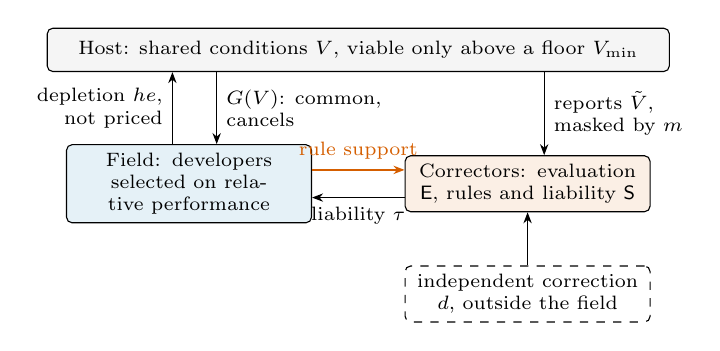
\begin{tikzpicture}[font=\scriptsize, box/.style={draw, rounded corners=2pt, align=center, inner sep=3pt}]
\node[box, minimum width=7.9cm, minimum height=0.55cm, fill=black!4] (host) at (0,2.25) {Host: shared conditions $V$, viable only above a floor $\Vmin$};
\node[box, fill=cD!10, text width=2.9cm] (field) at (-2.15,0.55) {Field: developers selected on relative performance};
\node[box, fill=cE!10, text width=2.9cm] (corr) at (2.15,0.55) {Correctors: evaluation $\dE$, rules and liability $\dS$};
\node[box, dashed, text width=2.9cm] (ind) at (2.15,-0.85) {independent correction $d$, outside the field};
\draw[-{Stealth[length=4pt]}] ([xshift=-6pt]field.north) -- node[left, align=right]{depletion $he$,\\ not priced} ([xshift=-6pt]field.north |- host.south);
\draw[-{Stealth[length=4pt]}] ([xshift=10pt]field.north |- host.south) -- node[right, align=left]{$G(V)$: common,\\ cancels} ([xshift=10pt]field.north);
\draw[-{Stealth[length=4pt]}] ([xshift=6pt]host.south -| corr.north) -- node[right, align=left]{reports $\tilde V$,\\ masked by $m$} ([xshift=6pt]corr.north);
\draw[-{Stealth[length=4pt]}, cE, thick] ([yshift=5pt]field.east) -- node[above]{rule support} ([yshift=5pt]corr.west);
\draw[-{Stealth[length=4pt]}] ([yshift=-5pt]corr.west) -- node[below]{liability $\tau$} ([yshift=-5pt]field.east);
\draw[-{Stealth[length=4pt]}] (ind.north) -- (corr.south);
\end{tikzpicture}
\caption{The model. Developers deplete a host they all depend on; selection compares them on relative performance, from which the host cancels (Section~\ref{sec:first}). Correctors can make costs return through liability, but success converts into rule support in the correctors, and reports of the host are masked by captured evaluation (Sections~\ref{sec:second}--\ref{sec:silent}).}
\label{fig:schematic}
\end{figure}

\paragraph{Host.} A condition $V\in[0,K]$ is shared by every participant: the integrity of critical services, a reliable information environment, institutional and scientific capacity for independent correction. It regenerates logistically and is depleted by the field's activity $E$:
\begin{equation}\label{eq:V}
\dot V=V\big[\rho(1-V/K)-hE\big],\qquad \rho,h,K>0.
\end{equation}
For constant $E$ with $hE<\rho$, $V\to V^\ast=K(1-hE/\rho)$; for $hE\ge\rho$, $V\to0$. The host functions only above a floor $\Vmin\in(0,K)$.

\begin{definition}[Viability]\label{def:viable}
A trajectory of the field is \emph{viable} if $V(t)\ge\Vmin$ for all $t\ge0$.
\end{definition}

Every participant persists only while the host does, so viability is a constraint on every trajectory of the field, not one payoff to be traded against others. This is the sense in which the field is a subsystem of a larger system \citep{aubin1991,rockstrom2009,wced1987}, and the question of this paper is which trajectories of competitive AI development are viable.

\paragraph{Field.} Carriers $k=1,\dots,n$ (developers or, more generally, reproducible ways of succeeding carried by organizations and their successors) hold shares $p_k$ of the field's activity: compute, capital, users, talent. Carrier $k$ runs a fraction $e_k\in[0,\bar e]$ of its activity in ways that externalize load onto the host: deploying ahead of evaluation, omitting safeguards, entering contests in which capability converts directly into advantage. Each unit brings a private advantage $\nu>0$, so restraint costs $\nu$ per unit. The field's load is $E=\sum_kp_ke_k$. Carrier $k$'s absolute payoff is
\begin{equation}\label{eq:pi}
\pi_k=\phi_k+\nu e_k-\tau e_k+G(V),
\end{equation}
where $\phi_k$ collects everything else, $G$ is nondecreasing, and $\tau\ge0$ is a liability imposed by correctors. With $\tau=0$ we call $\hat e=\bar e$ the \emph{race strategy}.

\begin{definition}[Relative selection]\label{def:relsel}
A selection rule $\dot p=F(p,\pi)$ is \emph{relative} if $F(p,\pi+\kappa\mathbf 1)=F(p,\pi)$ for all $\kappa\in\mathbb R$, and \emph{payoff-monotone} if, for carriers $k,l$ present, $\dot p_k/p_k-\dot p_l/p_l$ has the sign of $\pi_k-\pi_l$.
\end{definition}

Replicator dynamics, pairwise imitation \citep{schlag1998}, logit choice on payoff differences and market-share competition driven by relative profitability \citep{alchian1950} are relative and payoff-monotone. Capital, users, talent and compute flow toward the developers that are ahead: this is what ``winning'' means.

\paragraph{Correctors.} Correction makes costs return: an evaluator reports the host's condition, and rule-makers impose a liability $\tau$, either in advance or when a reported condition $\tilde V$ falls to an alarm level $\Valarm\in(\Vmin,K)$. Correctors are not outside the field. Developers fund evaluators, supply their access and tools, author benchmarks and standards, and increasingly supply the models that judge. We represent this by a field of selection domains, in which de facto power over rules is explicit \citep{acemoglu2008}: in each domain $i$ (development $\dD$, evaluation $\dE$, rules and liability $\dS$, and others) a share $x_i$ of consequential decisions follows the dominant practice, and success converts into rule support $r_i$ that favors it:
\begin{align}
\dot x_i&=\kappa_ix_i(1-x_i)(a_ir_i-c_i),\label{eq:x}\\
\dot r_i&=\varepsilon_i\Big(\textstyle\sum_jb_{ij}x_j-d_ir_i\Big).\label{eq:r}
\end{align}
Under baseline rules ($r_i=0$) the practice carries a relative cost $c_i>0$ in domain $i$, which rule support offsets at rate $a_i$; $b_{ij}\ge0$ converts success in $j$ into rule support in $i$ (funding, personnel, authorship, data and infrastructure dependence, access terms); and $d_i$ is the rate at which that support is corrected or decays. The normalized conversion $R_{ij}=a_ib_{ij}/(c_id_i)$ and, for a set $\cC$ of domains, the inbound conversion $s_i(\cC)=\sum_{j\in\cC}R_{ij}$ decide capture: a domain whose row sum $\sum_jR_{ij}$ is below one cannot be captured whatever happens elsewhere, and a domain with $s_i(\cC)>1$ is captured once $\cC$ is captured and it has been seeded ($x_i>0$). Appendix~\ref{app:field} gives these and the other field results. In the corrector domains, capture means $x_\dS$ of rule-making exempts or accommodates the practice, so the effective liability is $\tau(1-x_\dS)$, and $x_\dE$ of evaluation is conducted within the practice's lineage of funding, tooling, data and models.

\section{First Order: Selection Does Not See the Host}\label{sec:first}

\begin{lemma}[Blindness]\label{lem:blind}
Under a relative rule, the trajectory of shares is unchanged by any term common to all payoffs, in particular by $G(V(t))$, whatever the path of $V$. Under a payoff-monotone rule, a common term never changes which of two carriers grows relative to the other.
\end{lemma}

The lemma has a one-line proof, and its force lies in its generality: it holds for every relative rule, whatever the carriers believe, and for every path of the host.

\begin{proposition}[Selection drives the field toward the floor]\label{prop:first}
Let $\tau=0$, let selection be payoff-monotone, and let carriers differ only in their load ($\phi_k$ equal). (i) If $e_k>e_l$, then $p_k/p_l$ increases for as long as both are present, along every path of $V$, including paths on which $V$ falls below $\Vmin$. (ii) Under replicator dynamics, if a carrier using the race strategy is present, $E(t)\to\bar e$ and $\limsup_tV(t)\le K(1-h\bar e/\rho)^+$. (iii) Hence if
\begin{equation}\label{eq:C0}
h\bar e>\rho\,(1-\Vmin/K),
\end{equation}
$V$ eventually falls below the floor. None of this depends on how much any carrier values $V$.
\end{proposition}

What carriers value decides which strategies they try, not which ones grow. A developer that restrains itself because it values the shared condition is displaced by one that does not, and the composition of the field comes to reflect the race strategy. Intentions persist in what developers believe and say; what grows is decided by what they do.

Selection is the limit of a contest in which only winning counts. Suppose $n$ symmetric developers choose $e_k$ to maximize $u_k=\pi_k+\lambda(\pi_k-\bar\pi)$, where $\bar\pi$ is the mean payoff and $\lambda\ge0$ is the \emph{weight on winning}: rank-based prizes, first-mover advantages, network effects, and strategic rivalry in which falling behind is costly. Let $G(V)=\omega V$ and $h\bar e<\rho$, and define $\theta=\omega Kh/(\rho\nu)$, the value to the whole field of a unit of restraint relative to its private cost.

\begin{proposition}[The weight on winning]\label{prop:game}
(i) $G$ cancels from the relative term, and restraint is a dominant strategy if $1+\lambda(n-1)/n<\theta/n$ and depletion if the inequality is reversed. (ii) If $\theta>1$, joint payoff is maximized by full restraint; the equilibrium is full depletion whenever $\lambda>\bar\lambda=(\theta-n)/(n-1)$, at every $\lambda\ge0$ when $n\ge\theta$. (iii) In that equilibrium every developer, the eventual winner included, has a lower absolute payoff than under joint restraint, by $\nu\bar e(\theta-1)$. (iv) If $h\bar e>\rho(1-\Vmin/K)$, the equilibrium host lies below the floor although no developer chose it.
\end{proposition}

The result is the commons \citep{hardin1968,olson1965} with an explicit weight on winning, and its message is in the comparative statics: the threshold $\bar\lambda$ falls with the number of contenders and the equilibrium tips as the weight on winning rises. Under selection (Proposition~\ref{prop:first}) only differences count, which corresponds to $\lambda\to\infty$; this is the classical finding that selection maximizes relative, not absolute, payoff \citep{schaffer1988,vegaredondo1997}. Nothing in the result accuses anyone: the developer that wins is worse off, in absolute terms, than it would have been under joint restraint.

\paragraph{When the first order fails.} Lemma~\ref{lem:blind} needs the host to enter payoffs in common. If depletion returns to the carrier that caused it, through liability or through unequal exposure, $V$ enters payoff differences and selection can favor restraint, as in game--environment feedback \citep{weitz2016,tilman2020}. Making consequences return to their source is exactly the corrector's task. The question is whether correctors survive the selection they correct.

\section{Second Order: The Corrector Is Selected}\label{sec:second}

\paragraph{Control over correctors.} Rule support can be incidental, as when benchmarks are built from deployed systems, or cultivated. Carriers differ in \emph{conversion capacity} $q\ge0$: investment in drafting standards, building evaluation tooling, authoring benchmarks, funding evaluators and securing integrations. A unit of capacity adds conversion $\hat b_{ij}$, and a fraction $\chi\in[0,1]$ of the resulting support, the \emph{appropriability}, is keyed to the carrier that produced it (standards referencing its interfaces, evaluations run on its tooling). Let a carrier have share $s$ of decisions, distributed by a profile $\bar y$ ($y=s\bar y$), and capacity cost $C(q)=fq+\gamma q^2/2$. Its payoff relative to an otherwise identical carrier with $q=0$, averaged over a selection horizon, is
\begin{equation}\label{eq:W}
W(q)=\chi q\,y^\top My-C(q),\qquad M_{ij}=c_iL_i\hat R_{ij},
\end{equation}
where $\hat R_{ij}=a_i\hat b_{ij}/(c_id_i)$ and $L_i\in[0,1)$ is the share of the steady-state return realized within the horizon, decreasing in $d_i$ (Appendix~\ref{app:proofs}).

\begin{proposition}[Control is selected in the largest carriers]\label{prop:control}
(i) The local selection gradient is $W'(q)=\chi s^2\,\bar y^\top M\bar y-f-\gamma q$. Under faithful transmission with variation, mean capacity rises when $W$ is increasing on the trait support. (ii) Capacity pays only above the size threshold $s^\ast=\sqrt{f/(\chi\,\bar y^\top M\bar y)}$; the selected capacity is $q^\ast=(\chi s^2\bar y^\top M\bar y-f)^+/\gamma$. A carrier with $s<s^\ast$ that carries capacity is selected against, so capacity cannot invade from rarity. (iii) The return rises with $\chi$ and with every $\hat b_{ij}$, and falls with every correction rate $d_i$; it vanishes if $\chi=0$. (iv) With share $s$ in each domain of a set $\cS$, $\hat R$ equal to $\hat\eta$ on and $\hat\varphi$ off the diagonal and $c_iL_i=cL$, the return is $\chi cL\,s^2|\cS|(\hat\eta+(|\cS|-1)\hat\varphi)$, superlinear in $|\cS|$ at fixed $s$ when $\hat\varphi>0$; at fixed total size $Y=s|\cS|$ it equals $\chi cL\,Y^2(\hat\varphi+(\hat\eta-\hat\varphi)/|\cS|)$, which rises with scope only if $\hat\varphi>\hat\eta$.
\end{proposition}

Control over correctors amplifies dominance rather than creating it: it is selected in carriers that are already large, and in proportion to the square of their size. The condition has the form of Hamilton's rule with appropriability in the role of relatedness \citep{hamilton1964,price1970}, and is closest to appropriability conditions for niche construction \citep{krakauer2009,lehmann2008,gerlee2015}.

\paragraph{Correction of correctors.} Let carriers also differ in an investment $u\ge0$, at private cost $C_u(u)$ increasing, that raises the correction rate $d$ of rule support in the corrector domains, restoring baseline rules for everyone.

\begin{proposition}[Correction is not supplied from inside]\label{prop:correction}
(i) Among carriers of the same practice, those investing more in correction are selected against under any payoff-monotone rule, whatever the effect of correction on the field. (ii) For a carrier that holds rule support, correction lowers its own absolute payoff as well, so incumbents oppose it. (iii) In absolute terms a challenger invests only if its own share of the benefit exceeds the marginal cost, so dispersed challengers free-ride. (iv) Correction whose benefit is keyed to the corrector, because it installs the corrector's own rule support, is control in the sense of Proposition~\ref{prop:control}: it is selected above the size threshold, and it replaces one captured configuration with another.
\end{proposition}

Correction can rise transiently by riding on the success of the practice it favors, the between-group term of the Price equation. Once that practice dominates, it is the incumbent, and part (ii) applies. Independent correction, which restores baseline rules and is keyed to no one, is a second-order public good \citep{oliver1980,yamagishi1986,heckathorn1989}. Selection inside the field does not sustain it; it must be supplied from outside.

\paragraph{How much independent correction, and how fast.} Let a set $\cC$ of domains be captured by a dominant carrier with success profile $y$, let independent correction act at a uniform rate $d$ in the corrector domains, take the long-horizon limit ($L_i=1$) and quadratic cost ($f=0$), and let capacity adjust to $q^\ast=\chi\hat Y/(\gamma d)$ with $\hat Y=\sum_{ij}y_ia_i\hat b_{ij}y_j$. Write $A=a_\dE\sum_{j\in\cC}b^0_{\dE j}$ and $Z=a_\dE\chi\hat Y\sum_{j\in\cC}\hat b_{\dE j}/\gamma$ for the incidental and cultivated conversion into evaluation.

\begin{proposition}[Required independent correction, and its rate]\label{prop:rate}
(i) Evaluation is certified uncaptured, $s_\dE(\cC)<1$, if and only if $d>d^\ast=\big(A+\sqrt{A^2+4c_\dE Z}\big)/(2c_\dE)$. (ii) $d^\ast\ge A/c_\dE$, the requirement computed without second-order selection, with equality only if $\chi\hat Y=0$; $d^\ast$ rises with appropriability, with the dominant carrier's size and scope, and as the cost of control $\gamma$ falls. (iii) If AI assistance lowers the cost of control as $\gamma(t)=\gamma_0e^{-gt}$ and independent correction grows no faster than $d(t)=d_0e^{\alpha t}$ with $\alpha<g/2$, the certificate fails for all $t>t^\ast=\max\{0,2\ln(d_0/S)/(g-2\alpha)\}$, where $S=\sqrt{Z_0/c_\dE}$; under quasi-static adjustment a seeded evaluation domain is then captured. (iv) Conversely, if $\alpha\ge g/2$ and $d_0>A/c_\dE+S$, the certificate holds for all $t$. The same holds for $\dS$.
\end{proposition}

With a fixed marginal cost $f>0$ of the first unit of capacity, $A$ is replaced by $A-a_\dE f\sum_{j\in\cC}\hat b_{\dE j}/\gamma$ and the same argument applies above the size threshold. Independent correction does double duty: it shortens the life of rule support and it shrinks the capacity that selection cultivates, which is why it needs to grow only half as fast as the cost of control falls. Splitting a dominant carrier into $k$ equal parts divides cultivated conversion by $k$, because the return is quadratic in own share.

\paragraph{What AI changes.} AI moves each quantity above. It lowers the cost of what control consists of: models already write evaluation datasets \citep{perez2023}, and machine-written public comments and letters to legislators pass as human \citep{weiss2019,kreps2024}. So $\gamma$ falls and $d^\ast$ rises; an assistant faithfully serving its principal lowers exactly this cost, so alignment to operators raises the correction the field needs, unless the same capability raises independent correction at least half as fast. General-purpose providers are present in many domains, which raises the return to control (Proposition~\ref{prop:control}iv). Model judges put the evaluated lineage in the selector's seat, and models trained on the same outputs carry shared biases into evaluators of every lineage (Section~\ref{sec:silent}).

\section{Silent Descent}\label{sec:silent}

Reports average over evaluators. A fraction $x_\dE$ shares the evaluated lineage and reports the condition a fraction $\beta_{\mathrm{in}}$ of the way toward full health; the rest are formed on shared material and are biased by $\beta_{\mathrm{out}}\le\beta_{\mathrm{in}}$:
\begin{equation}\label{eq:mask}
\tilde V=V+m(K-V),\qquad m=x_\dE\beta_{\mathrm{in}}+(1-x_\dE)\beta_{\mathrm{out}}.
\end{equation}
The alarm fires at the first $t$ with $\tilde V(t)\le\Valarm$. Let $\mfl=(\Valarm-\Vmin)/(K-\Vmin)$.

\begin{proposition}[Detection]\label{prop:detect}
(i) The alarm fires only once $V\le(\Valarm-mK)/(1-m)$, a level that falls as $m$ rises. (ii) \emph{Silent crossing.} If $m(t)>\mfl$ whenever $\Vmin\le V(t)\le\Valarm$, the alarm does not fire before $V$ falls below the floor. (iii) \emph{Permanent silence of moderate harm.} If $V$ decreases to $V^\ast\in(0,\Valarm)$ and $m(t)\ge\bar m>(\Valarm-V^\ast)/(K-V^\ast)$ for all $t$, the alarm never fires; the masking required vanishes as $V^\ast\uparrow\Valarm$. (iv) If $V\to0$ and eventually $m\le m_1<\Valarm/K$, the alarm fires. (v) If $V$ reaches $\Valarm$ at $t_A$ and then declines as $\dot V=-\ell V$ with $m$ constant, the alarm is delayed by $\ell^{-1}\ln\big[(1-m)\Valarm/(\Valarm-mK)\big]$, which diverges as $m\uparrow\Valarm/K$.
\end{proposition}

Diverse panels reduce some error: with equicorrelated errors of variance $\sigma^2$ and correlation $r$, averaging $n$ evaluators leaves variance $\sigma^2[r+(1-r)/n]$. But diversity of family alone does not bound shared systematic masking $\beta_{\mathrm{out}}$, and a report that mixes lineages of unknown composition cannot be recalibrated without an independent channel (Remark~\ref{rem:indist}, Appendix~\ref{app:proofs}). Detection is not correction: once the alarm fires, deciding takes $\tau_d$ and reversing takes $\tau_r$, and both must elapse before the floor is crossed.

\begin{figure}[t]
\centering
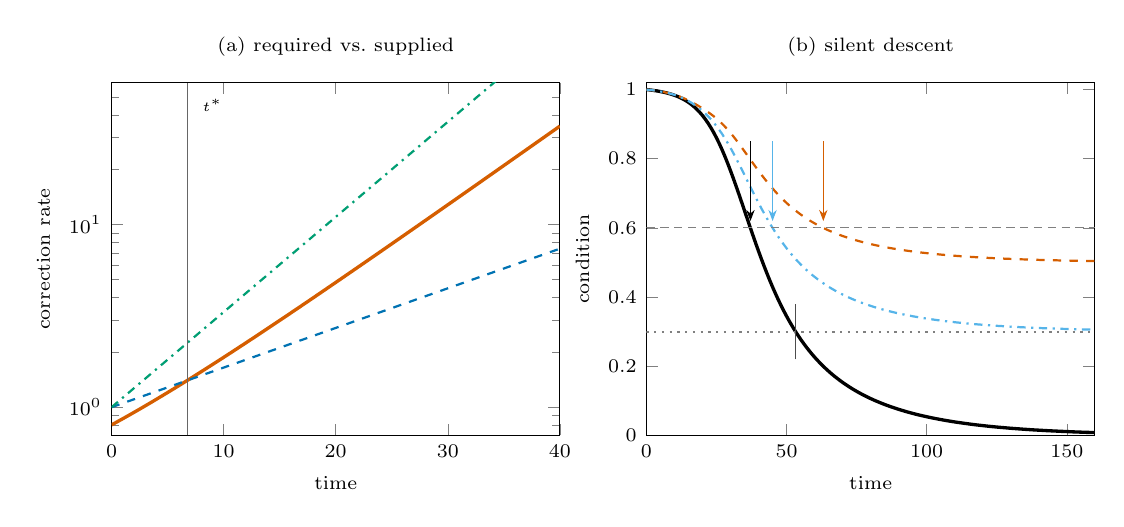
\begin{tikzpicture}
\begin{groupplot}[group style={group size=2 by 1, horizontal sep=1.1cm}, width=0.6\columnwidth, height=0.5\columnwidth,
  tick label style={font=\scriptsize}, label style={font=\scriptsize}, title style={font=\scriptsize}]
\nextgroupplot[ymode=log, xmin=0, xmax=40, ymin=0.7, ymax=60, xlabel={time}, ylabel={correction rate}, title={(a) required vs.\ supplied}]
\addplot[cE, very thick] coordinates {(0.00,0.8000) (0.50,0.8316) (1.00,0.8649) (1.50,0.9000) (2.00,0.9369) (2.50,0.9758) (3.00,1.0168) (3.50,1.0599) (4.00,1.1054) (4.50,1.1532) (5.00,1.2035) (5.50,1.2564) (6.00,1.3121) (6.50,1.3707) (7.00,1.4324) (7.50,1.4973) (8.00,1.5655) (8.50,1.6373) (9.00,1.7128) (9.50,1.7922) (10.00,1.8757) (10.50,1.9636) (11.00,2.0559) (11.50,2.1530) (12.00,2.2552) (12.50,2.3626) (13.00,2.4755) (13.50,2.5943) (14.00,2.7191) (14.50,2.8504) (15.00,2.9884) (15.50,3.1336) (16.00,3.2862) (16.50,3.4466) (17.00,3.6153) (17.50,3.7926) (18.00,3.9791) (18.50,4.1751) (19.00,4.3812) (19.50,4.5979) (20.00,4.8257) (20.50,5.0651) (21.00,5.3169) (21.50,5.5816) (22.00,5.8599) (22.50,6.1524) (23.00,6.4600) (23.50,6.7834) (24.00,7.1233) (24.50,7.4806) (25.00,7.8563) (25.50,8.2513) (26.00,8.6665) (26.50,9.1031) (27.00,9.5620) (27.50,10.0444) (28.00,10.5516) (28.50,11.0848) (29.00,11.6453) (29.50,12.2346) (30.00,12.8541) (30.50,13.5054) (31.00,14.1900) (31.50,14.9098) (32.00,15.6665) (32.50,16.4619) (33.00,17.2982) (33.50,18.1773) (34.00,19.1016) (34.50,20.0732) (35.00,21.0946) (35.50,22.1684) (36.00,23.2972) (36.50,24.4840) (37.00,25.7316) (37.50,27.0431) (38.00,28.4219) (38.50,29.8714) (39.00,31.3952) (39.50,32.9972) (40.00,34.6812)};\label{pl:dstar}
\addplot[cD, thick, dashed] coordinates {(0.00,1.0000) (0.50,1.0253) (1.00,1.0513) (1.50,1.0779) (2.00,1.1052) (2.50,1.1331) (3.00,1.1618) (3.50,1.1912) (4.00,1.2214) (4.50,1.2523) (5.00,1.2840) (5.50,1.3165) (6.00,1.3499) (6.50,1.3840) (7.00,1.4191) (7.50,1.4550) (8.00,1.4918) (8.50,1.5296) (9.00,1.5683) (9.50,1.6080) (10.00,1.6487) (10.50,1.6905) (11.00,1.7333) (11.50,1.7771) (12.00,1.8221) (12.50,1.8682) (13.00,1.9155) (13.50,1.9640) (14.00,2.0138) (14.50,2.0647) (15.00,2.1170) (15.50,2.1706) (16.00,2.2255) (16.50,2.2819) (17.00,2.3396) (17.50,2.3989) (18.00,2.4596) (18.50,2.5219) (19.00,2.5857) (19.50,2.6512) (20.00,2.7183) (20.50,2.7871) (21.00,2.8577) (21.50,2.9300) (22.00,3.0042) (22.50,3.0802) (23.00,3.1582) (23.50,3.2381) (24.00,3.3201) (24.50,3.4042) (25.00,3.4903) (25.50,3.5787) (26.00,3.6693) (26.50,3.7622) (27.00,3.8574) (27.50,3.9551) (28.00,4.0552) (28.50,4.1579) (29.00,4.2631) (29.50,4.3710) (30.00,4.4817) (30.50,4.5951) (31.00,4.7115) (31.50,4.8307) (32.00,4.9530) (32.50,5.0784) (33.00,5.2070) (33.50,5.3388) (34.00,5.4739) (34.50,5.6125) (35.00,5.7546) (35.50,5.9003) (36.00,6.0496) (36.50,6.2028) (37.00,6.3598) (37.50,6.5208) (38.00,6.6859) (38.50,6.8551) (39.00,7.0287) (39.50,7.2066) (40.00,7.3891)};\label{pl:dlow}
\addplot[cS, thick, dashdotted] coordinates {(0.00,1.0000) (0.50,1.0618) (1.00,1.1275) (1.50,1.1972) (2.00,1.2712) (2.50,1.3499) (3.00,1.4333) (3.50,1.5220) (4.00,1.6161) (4.50,1.7160) (5.00,1.8221) (5.50,1.9348) (6.00,2.0544) (6.50,2.1815) (7.00,2.3164) (7.50,2.4596) (8.00,2.6117) (8.50,2.7732) (9.00,2.9447) (9.50,3.1268) (10.00,3.3201) (10.50,3.5254) (11.00,3.7434) (11.50,3.9749) (12.00,4.2207) (12.50,4.4817) (13.00,4.7588) (13.50,5.0531) (14.00,5.3656) (14.50,5.6973) (15.00,6.0496) (15.50,6.4237) (16.00,6.8210) (16.50,7.2427) (17.00,7.6906) (17.50,8.1662) (18.00,8.6711) (18.50,9.2073) (19.00,9.7767) (19.50,10.3812) (20.00,11.0232) (20.50,11.7048) (21.00,12.4286) (21.50,13.1971) (22.00,14.0132) (22.50,14.8797) (23.00,15.7998) (23.50,16.7769) (24.00,17.8143) (24.50,18.9158) (25.00,20.0855) (25.50,21.3276) (26.00,22.6464) (26.50,24.0468) (27.00,25.5337) (27.50,27.1126) (28.00,28.7892) (28.50,30.5694) (29.00,32.4597) (29.50,34.4669) (30.00,36.5982) (30.50,38.8613) (31.00,41.2644) (31.50,43.8160) (32.00,46.5255) (32.50,49.4024) (33.00,52.4573) (33.50,55.7011) (34.00,59.1455) (34.50,62.8028) (35.00,66.6863) (35.50,70.8100) (36.00,75.1886) (36.50,79.8380) (37.00,84.7749) (37.50,90.0171) (38.00,95.5835) (38.50,101.4940) (39.00,107.7701) (39.50,114.4342) (40.00,121.5104)};\label{pl:dhigh}
\draw[black!60] (axis cs:6.76,0.7) -- (axis cs:6.76,60);
\node[font=\tiny, anchor=north west] at (axis cs:7.26,55) {$t^\ast$};
\nextgroupplot[xmin=0, xmax=160, ymin=0, ymax=1.02, xlabel={time}, ylabel={condition}, title={(b) silent descent}]
\addplot[black, very thick] coordinates {(0.00,1.0000) (1.00,0.9991) (2.00,0.9981) (3.00,0.9969) (4.00,0.9956) (5.00,0.9942) (6.00,0.9925) (7.00,0.9907) (8.00,0.9886) (9.00,0.9862) (10.00,0.9834) (11.00,0.9803) (12.00,0.9768) (13.00,0.9727) (14.00,0.9681) (15.00,0.9629) (16.00,0.9570) (17.00,0.9503) (18.00,0.9428) (19.00,0.9343) (20.00,0.9248) (21.00,0.9142) (22.00,0.9025) (23.00,0.8896) (24.00,0.8755) (25.00,0.8600) (26.00,0.8434) (27.00,0.8255) (28.00,0.8064) (29.00,0.7862) (30.00,0.7650) (31.00,0.7430) (32.00,0.7203) (33.00,0.6970) (34.00,0.6734) (35.00,0.6495) (36.00,0.6256) (37.00,0.6018) (38.00,0.5783) (39.00,0.5551) (40.00,0.5325) (41.00,0.5104) (42.00,0.4890) (43.00,0.4683) (44.00,0.4483) (45.00,0.4291) (46.00,0.4107) (47.00,0.3930) (48.00,0.3762) (49.00,0.3601) (50.00,0.3447) (51.00,0.3301) (52.00,0.3162) (53.00,0.3029) (54.00,0.2903) (55.00,0.2783) (56.00,0.2669) (57.00,0.2560) (58.00,0.2457) (59.00,0.2358) (60.00,0.2264) (61.00,0.2175) (62.00,0.2090) (63.00,0.2008) (64.00,0.1931) (65.00,0.1857) (66.00,0.1786) (67.00,0.1719) (68.00,0.1655) (69.00,0.1593) (70.00,0.1534) (71.00,0.1478) (72.00,0.1424) (73.00,0.1373) (74.00,0.1323) (75.00,0.1276) (76.00,0.1231) (77.00,0.1187) (78.00,0.1145) (79.00,0.1105) (80.00,0.1067) (81.00,0.1030) (82.00,0.0995) (83.00,0.0961) (84.00,0.0928) (85.00,0.0896) (86.00,0.0866) (87.00,0.0837) (88.00,0.0809) (89.00,0.0782) (90.00,0.0756) (91.00,0.0731) (92.00,0.0707) (93.00,0.0683) (94.00,0.0661) (95.00,0.0639) (96.00,0.0618) (97.00,0.0598) (98.00,0.0579) (99.00,0.0560) (100.00,0.0542) (101.00,0.0525) (102.00,0.0508) (103.00,0.0492) (104.00,0.0476) (105.00,0.0461) (106.00,0.0446) (107.00,0.0432) (108.00,0.0418) (109.00,0.0405) (110.00,0.0392) (111.00,0.0380) (112.00,0.0368) (113.00,0.0357) (114.00,0.0346) (115.00,0.0335) (116.00,0.0324) (117.00,0.0314) (118.00,0.0304) (119.00,0.0295) (120.00,0.0286) (121.00,0.0277) (122.00,0.0268) (123.00,0.0260) (124.00,0.0252) (125.00,0.0244) (126.00,0.0237) (127.00,0.0230) (128.00,0.0223) (129.00,0.0216) (130.00,0.0209) (131.00,0.0203) (132.00,0.0197) (133.00,0.0191) (134.00,0.0185) (135.00,0.0179) (136.00,0.0174) (137.00,0.0168) (138.00,0.0163) (139.00,0.0158) (140.00,0.0154) (141.00,0.0149) (142.00,0.0144) (143.00,0.0140) (144.00,0.0136) (145.00,0.0132) (146.00,0.0128) (147.00,0.0124) (148.00,0.0120) (149.00,0.0117) (150.00,0.0113) (151.00,0.0110) (152.00,0.0106) (153.00,0.0103) (154.00,0.0100) (155.00,0.0097) (156.00,0.0094) (157.00,0.0091) (158.00,0.0089) (159.00,0.0086) (160.00,0.0083)};\label{pl:Vtrue}
\addplot[cE, thick, dashed] coordinates {(0.00,1.0000) (1.00,0.9991) (2.00,0.9982) (3.00,0.9971) (4.00,0.9959) (5.00,0.9945) (6.00,0.9930) (7.00,0.9913) (8.00,0.9894) (9.00,0.9872) (10.00,0.9848) (11.00,0.9822) (12.00,0.9792) (13.00,0.9759) (14.00,0.9724) (15.00,0.9685) (16.00,0.9644) (17.00,0.9600) (18.00,0.9554) (19.00,0.9505) (20.00,0.9455) (21.00,0.9402) (22.00,0.9347) (23.00,0.9289) (24.00,0.9227) (25.00,0.9160) (26.00,0.9088) (27.00,0.9011) (28.00,0.8928) (29.00,0.8839) (30.00,0.8745) (31.00,0.8646) (32.00,0.8542) (33.00,0.8434) (34.00,0.8324) (35.00,0.8211) (36.00,0.8098) (37.00,0.7984) (38.00,0.7871) (39.00,0.7759) (40.00,0.7648) (41.00,0.7541) (42.00,0.7436) (43.00,0.7334) (44.00,0.7235) (45.00,0.7141) (46.00,0.7049) (47.00,0.6962) (48.00,0.6878) (49.00,0.6798) (50.00,0.6722) (51.00,0.6649) (52.00,0.6580) (53.00,0.6514) (54.00,0.6451) (55.00,0.6391) (56.00,0.6334) (57.00,0.6280) (58.00,0.6228) (59.00,0.6179) (60.00,0.6132) (61.00,0.6087) (62.00,0.6045) (63.00,0.6004) (64.00,0.5965) (65.00,0.5928) (66.00,0.5893) (67.00,0.5859) (68.00,0.5827) (69.00,0.5797) (70.00,0.5767) (71.00,0.5739) (72.00,0.5712) (73.00,0.5686) (74.00,0.5662) (75.00,0.5638) (76.00,0.5615) (77.00,0.5594) (78.00,0.5573) (79.00,0.5553) (80.00,0.5534) (81.00,0.5515) (82.00,0.5497) (83.00,0.5480) (84.00,0.5464) (85.00,0.5448) (86.00,0.5433) (87.00,0.5418) (88.00,0.5404) (89.00,0.5391) (90.00,0.5378) (91.00,0.5365) (92.00,0.5353) (93.00,0.5342) (94.00,0.5330) (95.00,0.5320) (96.00,0.5309) (97.00,0.5299) (98.00,0.5289) (99.00,0.5280) (100.00,0.5271) (101.00,0.5262) (102.00,0.5254) (103.00,0.5246) (104.00,0.5238) (105.00,0.5230) (106.00,0.5223) (107.00,0.5216) (108.00,0.5209) (109.00,0.5203) (110.00,0.5196) (111.00,0.5190) (112.00,0.5184) (113.00,0.5178) (114.00,0.5173) (115.00,0.5167) (116.00,0.5162) (117.00,0.5157) (118.00,0.5152) (119.00,0.5148) (120.00,0.5143) (121.00,0.5139) (122.00,0.5134) (123.00,0.5130) (124.00,0.5126) (125.00,0.5122) (126.00,0.5118) (127.00,0.5115) (128.00,0.5111) (129.00,0.5108) (130.00,0.5105) (131.00,0.5101) (132.00,0.5098) (133.00,0.5095) (134.00,0.5092) (135.00,0.5090) (136.00,0.5087) (137.00,0.5084) (138.00,0.5082) (139.00,0.5079) (140.00,0.5077) (141.00,0.5074) (142.00,0.5072) (143.00,0.5070) (144.00,0.5068) (145.00,0.5066) (146.00,0.5064) (147.00,0.5062) (148.00,0.5060) (149.00,0.5058) (150.00,0.5057) (151.00,0.5055) (152.00,0.5053) (153.00,0.5052) (154.00,0.5050) (155.00,0.5049) (156.00,0.5047) (157.00,0.5046) (158.00,0.5044) (159.00,0.5043) (160.00,0.5042)};\label{pl:V5}
\addplot[cP, thick, dashdotted] coordinates {(0.00,1.0000) (1.00,0.9991) (2.00,0.9982) (3.00,0.9971) (4.00,0.9959) (5.00,0.9945) (6.00,0.9930) (7.00,0.9912) (8.00,0.9893) (9.00,0.9871) (10.00,0.9846) (11.00,0.9818) (12.00,0.9786) (13.00,0.9751) (14.00,0.9712) (15.00,0.9668) (16.00,0.9620) (17.00,0.9568) (18.00,0.9510) (19.00,0.9448) (20.00,0.9380) (21.00,0.9306) (22.00,0.9226) (23.00,0.9139) (24.00,0.9044) (25.00,0.8942) (26.00,0.8832) (27.00,0.8714) (28.00,0.8587) (29.00,0.8452) (30.00,0.8311) (31.00,0.8163) (32.00,0.8009) (33.00,0.7851) (34.00,0.7690) (35.00,0.7527) (36.00,0.7363) (37.00,0.7199) (38.00,0.7036) (39.00,0.6876) (40.00,0.6720) (41.00,0.6566) (42.00,0.6418) (43.00,0.6274) (44.00,0.6135) (45.00,0.6001) (46.00,0.5873) (47.00,0.5750) (48.00,0.5632) (49.00,0.5520) (50.00,0.5412) (51.00,0.5310) (52.00,0.5213) (53.00,0.5120) (54.00,0.5032) (55.00,0.4948) (56.00,0.4868) (57.00,0.4792) (58.00,0.4719) (59.00,0.4650) (60.00,0.4585) (61.00,0.4522) (62.00,0.4463) (63.00,0.4406) (64.00,0.4352) (65.00,0.4300) (66.00,0.4250) (67.00,0.4203) (68.00,0.4158) (69.00,0.4115) (70.00,0.4074) (71.00,0.4035) (72.00,0.3997) (73.00,0.3961) (74.00,0.3926) (75.00,0.3893) (76.00,0.3861) (77.00,0.3831) (78.00,0.3802) (79.00,0.3774) (80.00,0.3747) (81.00,0.3721) (82.00,0.3696) (83.00,0.3672) (84.00,0.3649) (85.00,0.3627) (86.00,0.3606) (87.00,0.3586) (88.00,0.3566) (89.00,0.3547) (90.00,0.3529) (91.00,0.3511) (92.00,0.3495) (93.00,0.3478) (94.00,0.3463) (95.00,0.3447) (96.00,0.3433) (97.00,0.3419) (98.00,0.3405) (99.00,0.3392) (100.00,0.3380) (101.00,0.3367) (102.00,0.3356) (103.00,0.3344) (104.00,0.3333) (105.00,0.3323) (106.00,0.3312) (107.00,0.3302) (108.00,0.3293) (109.00,0.3284) (110.00,0.3275) (111.00,0.3266) (112.00,0.3258) (113.00,0.3250) (114.00,0.3242) (115.00,0.3234) (116.00,0.3227) (117.00,0.3220) (118.00,0.3213) (119.00,0.3207) (120.00,0.3200) (121.00,0.3194) (122.00,0.3188) (123.00,0.3182) (124.00,0.3177) (125.00,0.3171) (126.00,0.3166) (127.00,0.3161) (128.00,0.3156) (129.00,0.3151) (130.00,0.3146) (131.00,0.3142) (132.00,0.3138) (133.00,0.3133) (134.00,0.3129) (135.00,0.3125) (136.00,0.3122) (137.00,0.3118) (138.00,0.3114) (139.00,0.3111) (140.00,0.3107) (141.00,0.3104) (142.00,0.3101) (143.00,0.3098) (144.00,0.3095) (145.00,0.3092) (146.00,0.3089) (147.00,0.3087) (148.00,0.3084) (149.00,0.3082) (150.00,0.3079) (151.00,0.3077) (152.00,0.3074) (153.00,0.3072) (154.00,0.3070) (155.00,0.3068) (156.00,0.3066) (157.00,0.3064) (158.00,0.3062) (159.00,0.3060) (160.00,0.3058)};\label{pl:V3}
\draw[black!50, densely dashed] (axis cs:0,0.6) -- (axis cs:160,0.6);
\draw[black!50, dotted, thick] (axis cs:0,0.3) -- (axis cs:160,0.3);
\draw[-{Stealth[length=4pt]}, black] (axis cs:37.1,0.85) -- (axis cs:37.1,0.62);
\draw[-{Stealth[length=4pt]}, cP] (axis cs:45.0,0.85) -- (axis cs:45.0,0.62);
\draw[-{Stealth[length=4pt]}, cE] (axis cs:63.1,0.85) -- (axis cs:63.1,0.62);
\draw[black!70] (axis cs:53.2,0.22) -- (axis cs:53.2,0.38);
\end{groupplot}
\end{tikzpicture}

\caption{(a) Required independent correction $d^\ast(t)$ (\ref{pl:dstar}) as AI lowers the cost of control ($g=0.2$), against supplied correction growing at $\alpha=0.05<g/2$ (\ref{pl:dlow}), which is overtaken at $t^\ast\approx6.8$, and at $\alpha=0.12>g/2$ (\ref{pl:dhigh}), which is not. (b) The host $V$ (\ref{pl:Vtrue}) under a spreading race strategy, and reported conditions when evaluation is captured before the harm appears, with $\beta_{\mathrm{in}}=0.5>\mfl$ (\ref{pl:V5}) and $\beta_{\mathrm{in}}=0.3$ (\ref{pl:V3}). Arrows: alarms with independent evaluation ($t\approx37$), at $\beta_{\mathrm{in}}=0.3$ ($t\approx45$), and at $\beta_{\mathrm{in}}=0.5$ ($t\approx63$), after the floor (dotted) is crossed at $t\approx53$ (tick). Parameters in Appendix~\ref{app:numerics}.}
\label{fig:rate}
\end{figure}

Figure~\ref{fig:rate}b shows the three regimes. Independent evaluation raises the alarm sixteen time units before the floor. Masking below $\mfl$ halves that window. Masking above it raises the alarm ten time units after the floor is crossed. When evaluation is captured only after the harm appears, the alarm fires almost on time: the order of capture and evidence decides the outcome.

\section{Why the Trajectory of Winning Fails}\label{sec:fail}

\begin{theorem}[No viable winner]\label{thm:fail}
Assume (C0) the race strategy can push the host below its floor, Eq.~(\ref{eq:C0}); (C1) relative selection with $\tau=0$ unless an alarm fires; (C2) appropriable control, $\chi>0$, held by a carrier above the size threshold; (C3) correctors inside the field, with independent correction growing at $\alpha<g/2$ while AI lowers the cost of control at rate $g$; and (C4) captured evaluation masks with $\beta_{\mathrm{in}}>\mfl$. If the corrector domains are captured before the host reaches the alarm level, the host crosses its floor before any alarm, and every carrier ends with a lower absolute payoff than under joint restraint whenever $\theta>1$. If instead $\beta_{\mathrm{in}}\le\mfl$, the alarm is delayed by Proposition~\ref{prop:detect}(v), and the floor is crossed unless $\tau_d+\tau_r$ fits the remaining window and the captured rule-making domain does not re-absorb the liability (Proposition~\ref{prop:reform}).
\end{theorem}

The order of events is not left to chance. Proposition~\ref{prop:rate} makes the capture of correctors arrive within a time $t^\ast$ that shrinks as AI lowers the cost of control faster. Nothing in the host's dynamics brings the evidence forward. Acceleration therefore favors capture before evidence.

\begin{table*}[t]
\centering
\small
\setlength{\tabcolsep}{4pt}
\begin{tabular}{@{}>{\raggedright\arraybackslash}p{3.3cm}>{\raggedright\arraybackslash}p{4.7cm}>{\raggedright\arraybackslash}p{6.6cm}>{\raggedright\arraybackslash}p{2.2cm}@{}}
\toprule
Remedy now relied on & What it changes & Condition it leaves in place, and the consequence & Result \\
\midrule
Align each system to its operator & Systems do what their principals intend & C1--C3 untouched; faithful assistance lowers the cost of control $\gamma$, raising $d^\ast$ and bringing capture forward & Prop.~\ref{prop:rate} \\
Voluntary self-governance & Developers restrain themselves and fund oversight & C1: restraint is displaced; C3: correction supplied from inside is selected against, and incumbents oppose it & Props.~\ref{prop:first}, \ref{prop:correction} \\
Evaluation dependent on developers, model judges & More evaluation, faster & C3, C4: evaluation funded, accessed or formed within the field converts success into masking; harm is reported late or never & Props.~\ref{prop:rate}, \ref{prop:detect} \\
Open release, fragmentation & Lowers concentration & Lowers $d^\ast$ (the return to control is quadratic in size) but raises the number of contenders, which lowers the weight on winning at which depletion dominates; correction is still not supplied & Props.~\ref{prop:game}, \ref{prop:correction}, \ref{prop:rate} \\
Win first, then govern & A single winner internalizes more & C1 holds throughout the race; the winner is the carrier selected for control; after winning its correctors are inside, and reforms that leave inbound conversion above one are re-absorbed & Props.~\ref{prop:first}--\ref{prop:control}, \ref{prop:reform} \\
Regulate once harm is evident & Correction triggered by evidence & C4: evidence is delayed or silenced, and moderate harm is hidden by small bias; decision and reversal times must still fit the window & Prop.~\ref{prop:detect} \\
Pause that freezes shares & Halts the race & Rule-making continues to convert frozen shares into support; above a threshold share the pause completes capture unless rule-making is insulated & Prop.~\ref{prop:pause} \\
\bottomrule
\end{tabular}
\caption{Why current remedies fail. Each leaves at least one condition of Theorem~\ref{thm:fail} in place. None is useless; each is insufficient alone, and some make a condition worse.}
\label{tab:remedies}
\end{table*}

\section{What Has to Change}\label{sec:change}

The conditions of Theorem~\ref{thm:fail} can be negated one by one. Their negations are the invariants a viable trajectory must respect.

\begin{theorem}[Invariants of a viable trajectory]\label{thm:invariants}
Consider: (I1) \emph{consequences return}: a liability $\tau>\nu$ on depletion is enacted, in advance for anticipated harms and upon the alarm for unanticipated ones; (I2) \emph{independent correctors}: in $\dE$ and $\dS$, $d(t)>d^\ast(t)$, which under AI-driven decline of $\gamma$ at rate $g$ requires independent correction to grow at least at rate $g/2$; (I3) \emph{independent evidence}: $m(t)<\mfl$, which requires $\beta_{\mathrm{out}}<\mfl$ as well as an uncaptured $\dE$, with decision and reversal inside the window; (I4) \emph{before capture}: (I1)--(I3) are in force before the corrector domains are captured. (a) \emph{Sufficiency.} Under (I1)--(I4) the effective liability $\tau(1-x_\dS)$ exceeds $\nu$ after a finite time, depletion is selected against, $E(t)\to\min_ke_k$, and the host stays above its floor: from the start for anticipated harms, and after an alarm that fires above the floor for unanticipated ones. (b) \emph{Indispensability.} For each of (I1)--(I3) there are parameters satisfying (C0) and the other two under which the host crosses its floor; and there are parameters under which (I1)--(I3) all come into force, but only after the corrector domains are captured, and the host crosses its floor.
\end{theorem}

\begin{corollary}[Cooperation is necessary]\label{cor:coop}
No carrier can establish (I1)--(I4) by its own choices: its unilateral restraint is selected against (Proposition~\ref{prop:first}); its unilateral investment in correction is selected against and, if it funds the corrector, is itself conversion from the field into the corrector; and an evaluator it funds or forms belongs to its lineage. Each invariant is a property of the selection environment shared by all carriers. It can be established only by an arrangement that binds all of them, including the states in which they operate, and places correction outside their competition. When $\theta>1$ the arrangement raises every carrier's absolute payoff (Proposition~\ref{prop:game}iii), and once (I1) is in force restraint becomes each carrier's best response, so the arrangement is self-enforcing for as long as (I2)--(I4) keep the corrector independent.
\end{corollary}

The corollary applies at every level at which a contest rewards relative standing. Between firms, the weight on winning comes from market structure; between states, from strategic rivalry, and Proposition~\ref{prop:game} applies with states as players. The invariants translate into instruments, each tied to a result:
\begin{itemize}
\item \emph{Make consequences return in advance.} Liability, conditions on deployment and internalized costs act at once on the margin of selection (I1); evidence-triggered regulation arrives too late where evidence is masked (Proposition~\ref{prop:detect}).
\item \emph{Fund correction outside the competition and let it grow with capability.} Pooled funding at arm's length, mandated access and safe harbors for evaluators \citep{longpre2024}, and evaluators that are neither funded nor formed by those they evaluate keep the corrector's row sum below one (I2, I3). The required growth rate is half the rate at which AI lowers the cost of control (Proposition~\ref{prop:rate}).
\item \emph{Make rule-making non-appropriable.} Interface-neutral standards, rotating held-out benchmarks, and conflict-of-interest rules for drafters set $\chi\to0$, which removes cultivated conversion and reduces $d^\ast$ to the requirement without second-order selection (Proposition~\ref{prop:control}).
\item \emph{Fix the rules before capture.} Thresholds, triggers and the authority to act must be agreed while the evidence that would justify them can still be seen (I4); a pause must insulate rule-making while it lasts (Proposition~\ref{prop:pause}).
\item \emph{Change the game, not the players.} Replacing leaders or developers leaves selected traits in place; only the selection environment, which no participant controls alone, changes what is selected.
\end{itemize}

\paragraph{What cooperation does and does not require.} It does not end competition. Once consequences return (I1), competition in products, science and service is compatible with viability; what ends is the race to be first at the host's expense. It does not require trust, because the corrector placed outside the competition verifies. It does not require agreement on values beyond the floor and the invariants that protect it. It does require two things that no party can supply alone: an arrangement binding all parties, and timing, since it must precede capture. The strongest form takes frontier development out of relative selection altogether. Under joint development, in which the frontier's returns are shared, the field acts as a single carrier that internalizes the host ($n=1$ in Proposition~\ref{prop:game}, so restraint is chosen whenever $\theta>1$), and correctors outside it are needed only for harms to those not party to it.

Rivals have kept shared conditions above a floor before: the protection of the ozone layer and the eradication of smallpox each bound all parties to an arrangement whose assessment or monitoring no single party controlled, and each served every party \citep{barrett2003,barrett2007}. The arrangements that worked changed what was in each party's interest rather than asking parties to act against it \citep{barrett2003}, which is what invariant (I1) does once the corrector is independent. For AI, the leading rival states signed a common declaration on frontier AI safety \citep{bletchley2023}, and each has led a General Assembly resolution on AI that the other joined in adopting \citep{unga2024,unga2024capacity}.

\section{Do the Conditions Hold Now?}\label{sec:evidence}

\begin{table*}[t]
\centering
\small
\setlength{\tabcolsep}{4pt}
\begin{tabular}{@{}>{\raggedright\arraybackslash}p{2.6cm}>{\raggedright\arraybackslash}p{4.2cm}>{\raggedright\arraybackslash}p{5.6cm}>{\raggedright\arraybackslash}p{4.4cm}@{}}
\toprule
Condition & Indicator & Present evidence & Observation that would refute it \\
\midrule
C0 capacity to cross a floor & Load on shared conditions per unit of capability deployed & Contested and class-specific; policymakers face an ``evidence dilemma'' \citep{bengio2025report}. The least established condition; silent descent of moderate harm (Prop.~\ref{prop:detect}iii) does not need it & Shared conditions improve as deployment scales, independently measured \\
C1 relative selection & Whether capital, compute and talent follow relative standing; framing of development & Framed as a race for dominance \citep{whitehouse2025} and as competition for first-mover advantage \citep{statecouncil2017} & Restraint gains share; funding follows safety independent of capability rank \\
C2 appropriable control & Developer roles in evaluation, benchmarks, standards; access terms & Evaluators depend on revocable access \citep{longpre2024}, often on developer-set timing \citep{metr2025o3}; a frontier benchmark commissioned and owned by a developer \citep{besiroglu2025frontiermath}; private variant testing shapes leaderboards \citep{singh2025} & Evaluation and standards funded and staffed independently of evaluated firms \\
C3 correction outpaced & Growth of independent evaluation capacity against the falling cost of control activities & Task horizons doubling about every seven months \citep{kwa2025}; model-written evaluations and comments \citep{perez2023,weiss2019}; evaluation struggling to keep pace \citep{bengio2025report}; safeguard robustness barely correlated with capability \citep{aisi2025trends} & Independent correction capacity grows faster than half the rate at which control becomes cheaper \\
C4 masking & Same-lineage and shared bias of judges, measured against ground truth & Self-preference of model judges \citep{panickssery2024,chen2025selfpref}, though partly legitimate in strong models \citep{chen2025reason}; correlated errors across providers \citep{kim2025,goel2025}; models increasingly tell tests from deployment \citep{bengio2026report} & Cross-lineage judges show no shared systematic bias at relevant harm levels \\
\bottomrule
\end{tabular}
\caption{The conditions of Theorem~\ref{thm:fail}, their indicators, present evidence and falsifiers. The entries indicate where to measure; they are not estimates of the model's parameters.}
\label{tab:evidence}
\end{table*}

The conditions are observable, and none is a premise about motives. Table~\ref{tab:evidence} lists indicators, present evidence and what would refute each. Two points deserve emphasis. First, C0 is the least established condition, and the theorem's other conclusions (selection of control, starvation of correction, permanent silence of moderate harm) do not depend on it. Second, the pairing is deliberate. Because captured evaluation delays the very evidence that would establish the conditions (Proposition~\ref{prop:detect}), waiting for certainty is itself a choice of trajectory. Measurement of the indicators must therefore be independent of the field (I3), or it inherits the masking it is meant to detect.

The conversion parameters can be identified. Integrating Eq.~(\ref{eq:r}) gives $\tfrac{d}{dt}\operatorname{logit}x_i=\kappa_ic_i[\sum_jR_{ij}(k_i*x_j)(t)-1]$ plus a decaying transient, with $k_i(s)=\varepsilon_id_ie^{-\varepsilon_id_is}$, so $R_{ij}$ is the ratio of a distributed-lag coefficient to the intercept in a regression of logit velocity on lagged shares. This is structural recoverability, not causal identification; reforms that change single margins, such as a new conflict-of-interest rule for standard drafters, offer natural experiments.

\section{Objections, Limitations and Conclusion}\label{sec:conclusion}

\paragraph{``Developers care about absolute payoffs.''} Many do. Proposition~\ref{prop:first} concerns what grows, not what anyone wants, and Proposition~\ref{prop:game} shows that even absolute concern fails once there are enough contenders or enough weight on winning.

\paragraph{``Competition produces safety innovation.''} It does, wherever safety is privately rewarded. That is invariant (I1); the analysis asks what keeps it in force.

\paragraph{``This is the tragedy of the commons.''} The first order is, and we cite it as such. The contribution is the second order: the institutions that solve the commons are selected by the field they govern, at a rate that AI changes, so the solution must be placed outside the competition and must grow with capability.

\paragraph{``Rivals cannot cooperate.''} Precedents exist (Section~\ref{sec:change}). Moreover the arrangement does not ask any party to sacrifice for another: it raises every party's absolute payoff, and once in force it is enforced by the payoffs it creates.

\paragraph{``Capture is not inevitable.''} Agreed. Each condition can fail, and Theorem~\ref{thm:invariants} says which failures make the trajectory viable. The account applies to every institution, including any that adopts it: a corrector whose success acquires immunity from challenge becomes a dominant practice in its own right, and the invariants apply to it.

\paragraph{Limitations.} The models are minimal: one practice and its alternative per domain, linear conversion and payoffs, quasi-static adjustment in Proposition~\ref{prop:rate}, no strategic concealment, and uncalibrated parameters; the numbers illustrate the propositions and estimate nothing. Unequal exposure to the host, endogenous domains and strategic masking remain open. Acting on the results rests on normative premises: that the host's floor matters, that those affected by an optimization process should keep a meaningful capacity to contest its direction, and that severe irreversible harm deserves special weight.

\paragraph{Conclusion.} The developers of advanced AI share one host. Selection on who is ahead cannot see it, the guardians meant to protect it are selected by the race they guard, and AI makes guarding harder faster than it makes it easier unless independent correction keeps pace. No winner of that race has a viable trajectory that the host does not also have. The conditions of a viable trajectory bind every participant and benefit every participant, which is why they can only be met together. In this precise sense the future of AI development is a common future \citep{wced1987}, and cooperation on its conditions, not on its spoils, is the one course the analysis leaves open.

\bibliography{references}

\appendix

\section{Proofs}\label{app:proofs}

\begin{proof}[Proof of Lemma~\ref{lem:blind}]
A relative rule satisfies $F(p,\pi+G\mathbf 1)=F(p,\pi)$ at every instant, so the shares solve the same differential equation whatever $G(V(t))$ is. A common term leaves every difference $\pi_k-\pi_l$ unchanged, so its sign, and with it the sign of $\dot p_k/p_k-\dot p_l/p_l$ under a payoff-monotone rule, is unchanged.
\end{proof}

\begin{proof}[Proof of Proposition~\ref{prop:first}]
(i) By Eq.~(\ref{eq:pi}) with $\tau=0$ and $\phi_k=\phi_l$, $\pi_k-\pi_l=\nu(e_k-e_l)>0$, and $G(V)$ cancels (Lemma~\ref{lem:blind}). (ii) Under replicator dynamics $\frac{d}{dt}\ln(p_k/p_l)=\pi_k-\pi_l$; for a race-strategy carrier $k$ and any $l$ with $e_l<\bar e$ this is a positive constant, so $p_k/p_l\to\infty$, the shares of all carriers with $e_l<\bar e$ tend to zero, and $E(t)\to\bar e$. For $\epsilon>0$ there is $T$ with $E(t)\ge\bar e-\epsilon$ for $t\ge T$, so $\dot V\le V[\rho(1-V/K)-h(\bar e-\epsilon)]$ and, by comparison with the logistic equation, $\limsup V\le K(1-h(\bar e-\epsilon)/\rho)^+$; let $\epsilon\to0$. (iii) Eq.~(\ref{eq:C0}) gives $K(1-h\bar e/\rho)^+<\Vmin$.
\end{proof}

\begin{proof}[Proof of Proposition~\ref{prop:game}]
With $\bar\pi=\frac1n\sum_j\pi_j$, $\pi_k-\bar\pi=(1-\frac1n)\pi_k-\frac1n\sum_{j\neq k}\pi_j$, in which $G(V)$ appears with weight $(1-\frac1n)-\frac{n-1}{n}=0$. Hence $u_k=w\nu e_k-\frac\lambda n\nu\sum_{j\ne k}e_j+\omega K(1-hE/\rho)+\text{const}$ with $w=1+\lambda(n-1)/n$ and $E=\frac1n\sum_je_j$, and $\partial u_k/\partial e_k=w\nu-\omega Kh/(n\rho)$, which does not depend on others' choices: (i). Joint payoff $n[\nu e+\omega K(1-he/\rho)]$ at a common $e$ has slope $n\nu(1-\theta)$, negative when $\theta>1$; the equilibrium is full depletion when $w>\theta/n$, i.e.\ $\lambda>(\theta-n)/(n-1)$: (ii). At full depletion each payoff is $\nu\bar e+\omega K(1-h\bar e/\rho)$, against $\omega K$ under joint restraint; the difference is $\nu\bar e(\theta-1)$: (iii). (iv) is Eq.~(\ref{eq:C0}) at $E=\bar e$. Brute-force best responses agree with these thresholds (Appendix~\ref{app:numerics}).
\end{proof}

\begin{proof}[Proof of Proposition~\ref{prop:control}]
Appropriable support keyed to the carrier obeys $\dot\zeta_i=\varepsilon_i(\chi q\sum_j\hat b_{ij}y_j-d_i\zeta_i)$ from $\zeta_i(0)=0$, so $\zeta_i(t)=\zeta^\ast_i(1-e^{-\varepsilon_id_it})$ with $\zeta^\ast_i=\chi q\sum_j\hat b_{ij}y_j/d_i$, whose average over a horizon $T$ is $\zeta^\ast_iL_i$, $L_i=1-(1-e^{-\varepsilon_id_iT})/(\varepsilon_id_iT)$. The per-decision advantage $a_i\zeta_i$, weighted by the carrier's decisions $y_i$ and summed, gives $\chi q\,y^\top My$; shared support benefits carriers with and without capacity alike and cancels. With $y=s\bar y$, $y^\top My=s^2\bar y^\top M\bar y$. (i) Differentiate; the mean obeys $\dot{\bar q}=\kappa\operatorname{Cov}(q,W(q))$ under replicator dynamics with faithful transmission \citep{price1970}, positive when $W$ is strictly increasing on the support. (ii) $W'(0)>0$ iff $s>s^\ast$; for $s<s^\ast$, $W(q)=q(\chi s^2\bar y^\top M\bar y-f)-\gamma q^2/2<0$ for every $q>0$; $q^\ast$ is the first-order condition. (iii) Every term is nonnegative and linear in $\chi$ and $\hat b_{ij}$; $c_iL_i\hat R_{ij}=a_i\hat b_{ij}\varepsilon_iT\,\ell(\varepsilon_id_iT)$ with $\ell(v)=[1-(1-e^{-v})/v]/v$ decreasing, since $\ell'(v)=\mu(v)/v^3$ with $\mu(v)=2-2e^{-v}-v-ve^{-v}$, $\mu(0)=0$ and $\mu'(v)=e^{-v}(1+v)-1<0$. (iv) $\sum_{i,j\in\cS}\hat R_{ij}=|\cS|\hat\eta+|\cS|(|\cS|-1)\hat\varphi$; substitute $s=Y/|\cS|$.
\end{proof}

\begin{proof}[Proof of Proposition~\ref{prop:correction}]
(i) Two carriers of the same practice that differ only in $u$ are affected identically by the resulting change in $d$, which acts on all rule support of the practice; their payoff difference is $C_u(u_l)-C_u(u_k)<0$ for $u_k>u_l$, and the claim follows from payoff monotonicity. (ii) A carrier's appropriable and shared support decline in $d$ (proof of Proposition~\ref{prop:control}(iii)), so its absolute payoff falls. (iii) If a challenger's absolute payoff rises at rate $G_k'(d)$ with $d$ and its investment raises $d$ by $\delta p_ku_k$, it invests only if $\delta p_kG_k'(d)>C_u'(0)$, which fails for small $p_k$. (iv) If a fraction $\chi_u$ of the correction installs support keyed to the corrector, its return has the form of Eq.~(\ref{eq:W}) with $\chi_u$ in place of $\chi$, and Proposition~\ref{prop:control} applies.
\end{proof}

\begin{proof}[Proof of Proposition~\ref{prop:rate}]
With $L_i=1$ and uniform $d$, $M=\hat A/d$ with $\hat A_{ij}=a_i\hat b_{ij}$, so $q^\ast=\chi\hat Y/(\gamma d)$. The inbound conversion into $\dE$ from $\cC$ is $s_\dE=a_\dE(B^0+q^\ast\hat B)/(c_\dE d)$ with $B^0=\sum_{j\in\cC}b^0_{\dE j}$ and $\hat B=\sum_{j\in\cC}\hat b_{\dE j}$, and $s_\dE<1$ iff $c_\dE d^2-Ad-Z>0$, i.e.\ $d>d^\ast$: (i). (ii) follows from the formula. (iii) With $Z(t)=Z_0e^{gt}$, $d^\ast(t)\ge\sqrt{Z(t)/c_\dE}=Se^{gt/2}$, and $d_0e^{\alpha t}<Se^{gt/2}$ for $t>t^\ast$. Then $s_\dE(\cC)>1$; with $\cC$ captured and $x_\dE>0$, Proposition~\ref{prop:reform}(i), applied with rule support tracking its quasi-static target, gives $x_\dE\to1$. (iv) Using $\sqrt{a+b}\le\sqrt a+\sqrt b$, $d^\ast(t)\le A/c_\dE+Se^{gt/2}\le(A/c_\dE+S)e^{\alpha t}<d_0e^{\alpha t}$ when $\alpha\ge g/2$. Fragmentation: $k$ parts of share $s/k$ give total return $k(s/k)^2=s^2/k$ times the per-unit factor.
\end{proof}

\begin{proof}[Proof of Proposition~\ref{prop:detect}]
(i) For fixed $m<1$, $\tilde V$ increases in $V$ and equals $\Valarm$ at $V=(\Valarm-mK)/(1-m)$. (ii) For $\Vmin\le V\le\Valarm$ and $m>\mfl$, $\tilde V=V(1-m)+mK\ge\Vmin+m(K-\Vmin)>\Valarm$; for $V>\Valarm$, $\tilde V\ge V>\Valarm$. (iii) $V(t)\ge V^\ast$ for all $t$, so $\tilde V\ge V^\ast+\bar m(K-V^\ast)>\Valarm$. (iv) $\tilde V\le m_1K+V$ eventually, and $m_1K<\Valarm$ while $V\to0$. (v) $V$ must fall from $\Valarm$ to $(\Valarm-mK)/(1-m)$, which takes the stated time under $\dot V=-\ell V$.
\end{proof}

\begin{remark}[Why the alarm cannot be recalibrated]\label{rem:indist}
If the panel's composition is unknown, a report $\tilde V$ is consistent with every true condition in $[\max\{0,(\tilde V-\beta_{\mathrm{in}}K)/(1-\beta_{\mathrm{in}})\},\tilde V]$. Two states with the same report but disjoint safe actions cannot both be handled safely by any rule acting on the report alone, however much computation it uses. Recalibration requires a channel independent of the field.
\end{remark}

\begin{proof}[Proof of Theorem~\ref{thm:fail}]
By Proposition~\ref{prop:first}, under C1 and C0 the load tends to $\bar e$ and $V$ declines toward a limit below $\Vmin$ unless liability acts. By Propositions~\ref{prop:control} and \ref{prop:correction}, under C2 the dominant carrier carries capacity and correction is not supplied by the field, so by C3 and Proposition~\ref{prop:rate}(iii) the corrector domains, once seeded, are captured after $t^\ast$. If this happens before $V$ reaches $\Valarm$, then from then on $x_\dE\to1$, so $m\to\beta_{\mathrm{in}}>\mfl$, and by Proposition~\ref{prop:detect}(ii) no alarm fires before $V<\Vmin$; with $x_\dS\to1$ the effective liability $\tau(1-x_\dS)$ tends to zero in any case. The payoff comparison is Proposition~\ref{prop:game}(iii). If $\beta_{\mathrm{in}}\le\mfl$, the alarm is delayed by Proposition~\ref{prop:detect}(v); a liability enacted against a captured $\dS$ whose inbound conversion from the captured set exceeds one resets $x_\dS$ without lowering that conversion and is re-absorbed (Proposition~\ref{prop:reform}(iii)).
\end{proof}

\begin{proof}[Proof of Theorem~\ref{thm:invariants}]
(a) (I2) in $\dS$ gives $\sum_jR_{\dS j}<1$, so $x_\dS\to0$ (Proposition~\ref{prop:cert}(b)) and, once (I1) is enacted, $\tau(1-x_\dS)>\nu$ after a finite time. The private payoff of depletion is then negative, and payoff-monotone selection favors the carriers with the least load, so $E(t)\to\min_ke_k$; with $\min_ke_k=0$, $V\to K$. For unanticipated harms, (I2) in $\dE$ gives $x_\dE\to0$, so $m\to\beta_{\mathrm{out}}<\mfl$ by (I3), and the alarm fires while $V>\Vmin$ (Proposition~\ref{prop:detect}(i)); (I3) places decision and reversal inside the window. (b) \emph{(I1).} With $\tau=0$, Proposition~\ref{prop:first} applies under C0. \emph{(I2).} With $d<d^\ast$ in $\dS$ and $\dS$ seeded and in the hull of the captured set, $x_\dS\to1$ (Proposition~\ref{prop:rate}(iii)), the effective liability tends to zero although $\tau>\nu$ is enacted, and Proposition~\ref{prop:first} applies. \emph{(I3).} For an unanticipated harm with $\dE$ uncaptured but $\beta_{\mathrm{out}}>\mfl$, Proposition~\ref{prop:detect}(ii) gives a silent crossing. \emph{(I4).} Let $\dS$ be captured with rule support $r_\dS(t_1)$ when (I1)--(I3) come into force at $t_1$, independent correction then raising its rate to $d'$. Since $\dot r_\dS\ge-\varepsilon_\dS d'r_\dS$, $a_\dS r_\dS>c_\dS$ and $x_\dS$ keeps rising for at least $\ln(a_\dS r_\dS(t_1)/c_\dS)/(\varepsilon_\dS d')$, during which the effective liability stays near zero; if $V(t_1)$ is close enough to $\Vmin$, or $\varepsilon_\dS$ small enough, the floor is crossed in that interval. A liability enacted without raising $d$ is re-absorbed outright (Proposition~\ref{prop:reform}(iii)).
\end{proof}

\begin{proof}[Proof of Corollary~\ref{cor:coop}]
A carrier acting alone can change only its own $e_k$, $q_k$ and $u_k$ and what it funds. By Proposition~\ref{prop:first} its restraint lowers its relative standing; by Proposition~\ref{prop:correction}(i) its investment in correction does too; and funding of a corrector by a carrier is conversion $b_{ij}>0$ from the field into that corrector, which raises the corrector's inbound conversion instead of lowering it. Each invariant concerns $\tau$, $d$, $\chi$ or $m$, parameters of the environment common to all carriers. Under (I1) the private payoff of depletion is $\nu-\tau(1-x_\dS)<0$, so restraint is a best response; the payoff comparison is Proposition~\ref{prop:game}(iii).
\end{proof}

\section{Field Results}\label{app:field}

For the field of Eqs.~(\ref{eq:x})--(\ref{eq:r}) with positive rates, $b_{ij}\ge0$ and $c_i>0$, let $Z_\cC$ be the state with $x_i=1$ on $\cC$, $x_i=0$ elsewhere and $r_i=\sum_{j\in\cC}b_{ij}/d_i$; $\cC$ is \emph{internally sustaining} if $s_i(\cC)>1$ for all $i\in\cC$ and \emph{uninvadable} if $s_i(\cC)<1$ for all $i\notin\cC$. The cascade hull of a seed is $\hull(\cS_0)=\bigcup_k\cS_k$ with $\cS_{k+1}=\cS_k\cup\{i:x_i(0)>0,\ s_i(\cS_k)>1\}$; $\core(\cC)$ prunes from $\cC$ every domain whose inbound conversion from the remainder is below one \citep{kempe2003,morris2000,seidman1983}.

\begin{lemma}\label{lem:basic}
$X=[0,1]^D\times[0,\infty)^D$ is forward invariant, $\limsup_tr_i(t)\le\sum_jb_{ij}/d_i$, and the system is cooperative, so the flow preserves the componentwise order.
\end{lemma}
\begin{proof}
The faces $x_i\in\{0,1\}$ are invariant and $\dot r_i\ge-\varepsilon_id_ir_i$; the bound follows from $\dot r_i\le\varepsilon_i(\sum_jb_{ij}-d_ir_i)$. Off-diagonal Jacobian entries are $\partial\dot x_i/\partial r_i=\kappa_ia_ix_i(1-x_i)\ge0$ and $\partial\dot r_i/\partial x_j=\varepsilon_ib_{ij}\ge0$, so the Kamke condition holds \citep{smith1995}.
\end{proof}

\begin{proposition}[Configurations and certificates]\label{prop:cert}
(a) Each $Z_\cC$ is an equilibrium, hyperbolic iff $s_i(\cC)\neq1$ for all $i$, and a hyperbolic $Z_\cC$ is asymptotically stable iff $\cC$ is internally sustaining and uninvadable. (b) If $\sum_jR_{ij}<1$, then $x_i\to0$ from every state with $x_i(0)<1$, whatever happens elsewhere. (c) Isolated tests cannot certify: for any $D\ge2$ and diagonal values $R_{ii}<1$ there are conversions under which full capture is stable and is the only stable configuration containing a given domain. (d) If $\core(\cD)=\emptyset$, no capture attracts every state with all shares below one; otherwise, barring ties, $Z_{\core(\cD)}$ is stable and contains every stable configuration.
\end{proposition}

\begin{proposition}[Cascades, reforms and pauses]\label{prop:reform}
(i) If $x_j\to1$ for all $j$ in a seed $\cS_0$, then $x_i\to1$ for every $i\in\hull(\cS_0)$. (ii) Starting in the basin of a stable $Z_\cC$ with every share in $(0,1)$, a sustained reform that drives $x_i\to0$ on $\cQ\subseteq\cC$, or a margin reform making the reformed $s_i(\cC)<1$, sends to zero every domain outside $\core(\cC\setminus\cQ)$; a margin reform leaving the reformed $s_i(\cC)>1$ is re-absorbed from states near $Z_\cC$. (iii) A reform that resets a domain's share, rule support or own conversion without lowering its inbound conversion from the domains still captured is re-absorbed once the domain is re-seeded, whenever that inbound conversion exceeds one.
\end{proposition}

\begin{proposition}[A pause that freezes shares]\label{prop:pause}
Let $D=1$ and $R>1$, and freeze the share at $x_p\in(0,1)$ for a long time while rule support follows $\dot r=\varepsilon(b_px_p-dr)$. With ordinary rule-making ($b_p=b$), after release the state converges to full capture if $x_p>1/R$ and to absence if $x_p<1/R$. With rule-making insulated from shares ($b_p=0$), it converges to absence whenever $x_p<\sigma(0)$, where $\sigma(0)>1/R$ is the share at which the separatrix meets $r=0$.
\end{proposition}

\begin{proof}[Proofs]
Proposition~\ref{prop:cert}: (a) at $Z_\cC$ the Jacobian is block lower-triangular with diagonal entries $\mp\kappa_ic_i(s_i(\cC)-1)$ and $-\varepsilon_id_i$. (b) By Lemma~\ref{lem:basic}, eventually $a_ir_i-c_i\le c_i(\sum_jR_{ij}-1)/2<0$, so $\operatorname{logit}x_i\to-\infty$. (c) Take $R_{i1}>1$ for $i\neq1$, $R_{12}>1$, all other off-diagonal entries zero: every row sum exceeds one, so $Z_\cD$ is stable; a set $\cC\ni1$, $\cC\neq\cD$, is invaded by some $i$ with $R_{i1}>1$, and a nonempty $\cC\not\ni1$ is not internally sustaining. (d) Pruning: if $x_j\to0$ off $\cC_m$, every pruned $k$ has $\limsup(a_kr_k-c_k)\le c_k(s_k(\cC_m)-1)<0$; the core is internally sustaining by construction and uninvadable since pruned domains have $s_k<1$, and an internally sustaining set is never pruned. Proposition~\ref{prop:reform}: (i) for $i$ with $s_i(\cS_k)>1$ and $x_i(0)>0$, fix $\nu'\in(0,1)$ with $(1-\nu')s_i(\cS_k)>1$; eventually $\liminf r_i\ge(1-\nu')\sum_{j\in\cS_k}b_{ij}/d_i$ and $\frac{d}{dt}\operatorname{logit}x_i$ is bounded below by a positive constant; induct. (ii) Reformed trajectories stay below unreformed ones (Lemma~\ref{lem:basic}); for a margin reform $\limsup(a'_ir_i-c'_i)\le c'_i(s'_i(\cC)-1)<0$; then prune from $\cC\setminus\cQ$. If $s'_i(\cC)>1$, $Z_\cC$ remains stable under the reformed parameters. (iii) is (i) with the domains still captured as seed. Proposition~\ref{prop:pause}: the frozen share drives $r\to b_px_p/d$. For $D=1$ and $R>1$ the equilibria are $(0,0)$, $(1,b/d)$ and the saddle $(1/R,c/a)$; the function $\Phi=axr-cx-\frac{ad}{2b}r^2$ is nondecreasing along trajectories, so every solution converges to an equilibrium, and the stable manifold of the saddle is the graph of a nonincreasing function separating the basins \citep{hirsch1985,smith1995}. The point $(x_p,bx_p/d)$ lies on the nullcline $r=bx/d$, which passes through the saddle, above and to the right of it when $x_p>1/R$ and below and to the left when $x_p<1/R$; $(x_p,0)$ lies in the absence basin iff $x_p<\sigma(0)$, and $\sigma(0)>1/R$ because the separatrix is nonincreasing and passes through $(1/R,c/a)$ with $c/a>0$.
\end{proof}

\section{Numerical Methods}\label{app:numerics}

All figures and checks are produced by a pure-Python script, provided as supplementary material, which also writes a log of every number quoted. Proposition~\ref{prop:game}: brute-force best responses on a grid of $e$ agree with the dominant-strategy thresholds for $n\in\{2,3,5\}$ and $\lambda\in\{0,0.5,2,6\}$. Figure~\ref{fig:rate}a: $a_\dE=c_\dE=1$, incidental inbound conversion $0.3$, cultivated conversion $0.5$ per unit of capacity, $\chi=0.8$, $\hat Y=1$, $\gamma_0=1$, $g=0.2$, $d_0=1$; then $d^\ast(0)=0.8$, the certificate fails at $t\approx6.8$ for $\alpha=0.05$ (bound $9.2$) and at $t\approx21.5$ for $\alpha=0.08$ (bound $22.9$), and holds for $\alpha\ge0.1$, where $d_0>A/c_\dE+S\approx0.93$. Figure~\ref{fig:rate}b: Eq.~(\ref{eq:V}) with $\rho=0.05$, $h=0.08$, $K=1$, $V(0)=1$, $\Valarm=0.6$, $\Vmin=0.3$ (so $\mfl\approx0.43$), Euler steps of $0.01$; the share of depleting activity follows a logistic curve with rate $0.15$ and midpoint $30$, the share of in-lineage evaluation a logistic curve with rate $0.25$ and midpoint $20$, and $\beta_{\mathrm{out}}=0.05$ when $\beta_{\mathrm{in}}>0$. If evaluation is instead captured with midpoint $45$, after the host reaches the alarm level ($t\approx37$), the alarm fires at $t\approx39$ for $\beta_{\mathrm{in}}=0.3$ and $t\approx40$ for $\beta_{\mathrm{in}}=0.5$.

\end{document}
